%%
%  ******************************************************************************
%  * #file    Szablon_raportu_EN_Latex.tex
%  * #author  Adrian Wójcik   adrian.wojcik(at)put.poznan.pl
%  *          
%  * #commit  Patryk Kościk   koscikpatryk(at)gmail.com
%  *          Modified the template for Projekt przejsciowy purposes          
%  *          
%  * #version 1.0
%  * #date    09-Mar-2022
%  * #brief   PROJPRZEJ
%  *
%  ******************************************************************************
%%  
\documentclass[11pt, a4paper]{article}

\usepackage{SM_template}

% Wypełnijcie te dyrektywy zgodnie z waszym tematem
% \lab      -> NAZWA CZUJNIKA, np.: 'DHT22'
% \comment  -> Króciutki opis co to, np.: 'Cyfrowy budżetowy czujnik temperatury'
%

\lab{Moduł TTP223}
\comment{Pojemnościowy przycisk dotykowy}
\author{Antoni Borowski}
\addbibresource{bib/KY-018.bib}

% Absolutny zakaz dotykania tego tutaj bo jak dotkiecie to coś jebnie
\university{Politechnika Poznańska}
\faculty{Wydział Automatyki, Robotyki i Elektrotechniki}
\institute{Instytut Robotyki i Inteligencji Maszynowej}
\department{Zakład Sterowania i Elektroniki Przemysłowej}




%%
%
% Początek dokumentu
%
%%
\begin{document}

%% Strona tytułowa %%
\mainpage{{KY-018/front}}
\newpage

\section*{Opis elementu} \addcontentsline{toc}{section}{Wstęp}
Moduł TTP223 to pojemnościowy przycisk dotykowy. Działanie oparte jest na zjawisku oddziaływania pola elektrycznego z przewodnikami, zwłaszcza z ciałem ludzkim wypełnionym elektrolitami i otoczonym warstwą stratnego dielektryka w postaci skóry. Podzespołem elektronicznym, wytwarzającym pole elektryczne jest kondensator. Palec znajdujący się w brzegowym polu elektrycznym wprowadza do układu pewną pojemność, nazywaną powszechnie pojemnością dotykową. 
\vspace{0.5cm}
\begin{figure}[h!]
\centering
\begin{subfigure}{.5\textwidth}
  \centering
  \includegraphics[width=0.6\linewidth]{fig/KY-018/zdj_modułu/tył.png}
  \caption{Przód modułu}
  \label{fig:sub1}
\end{subfigure}%
\begin{subfigure}{.5\textwidth}
  \centering
  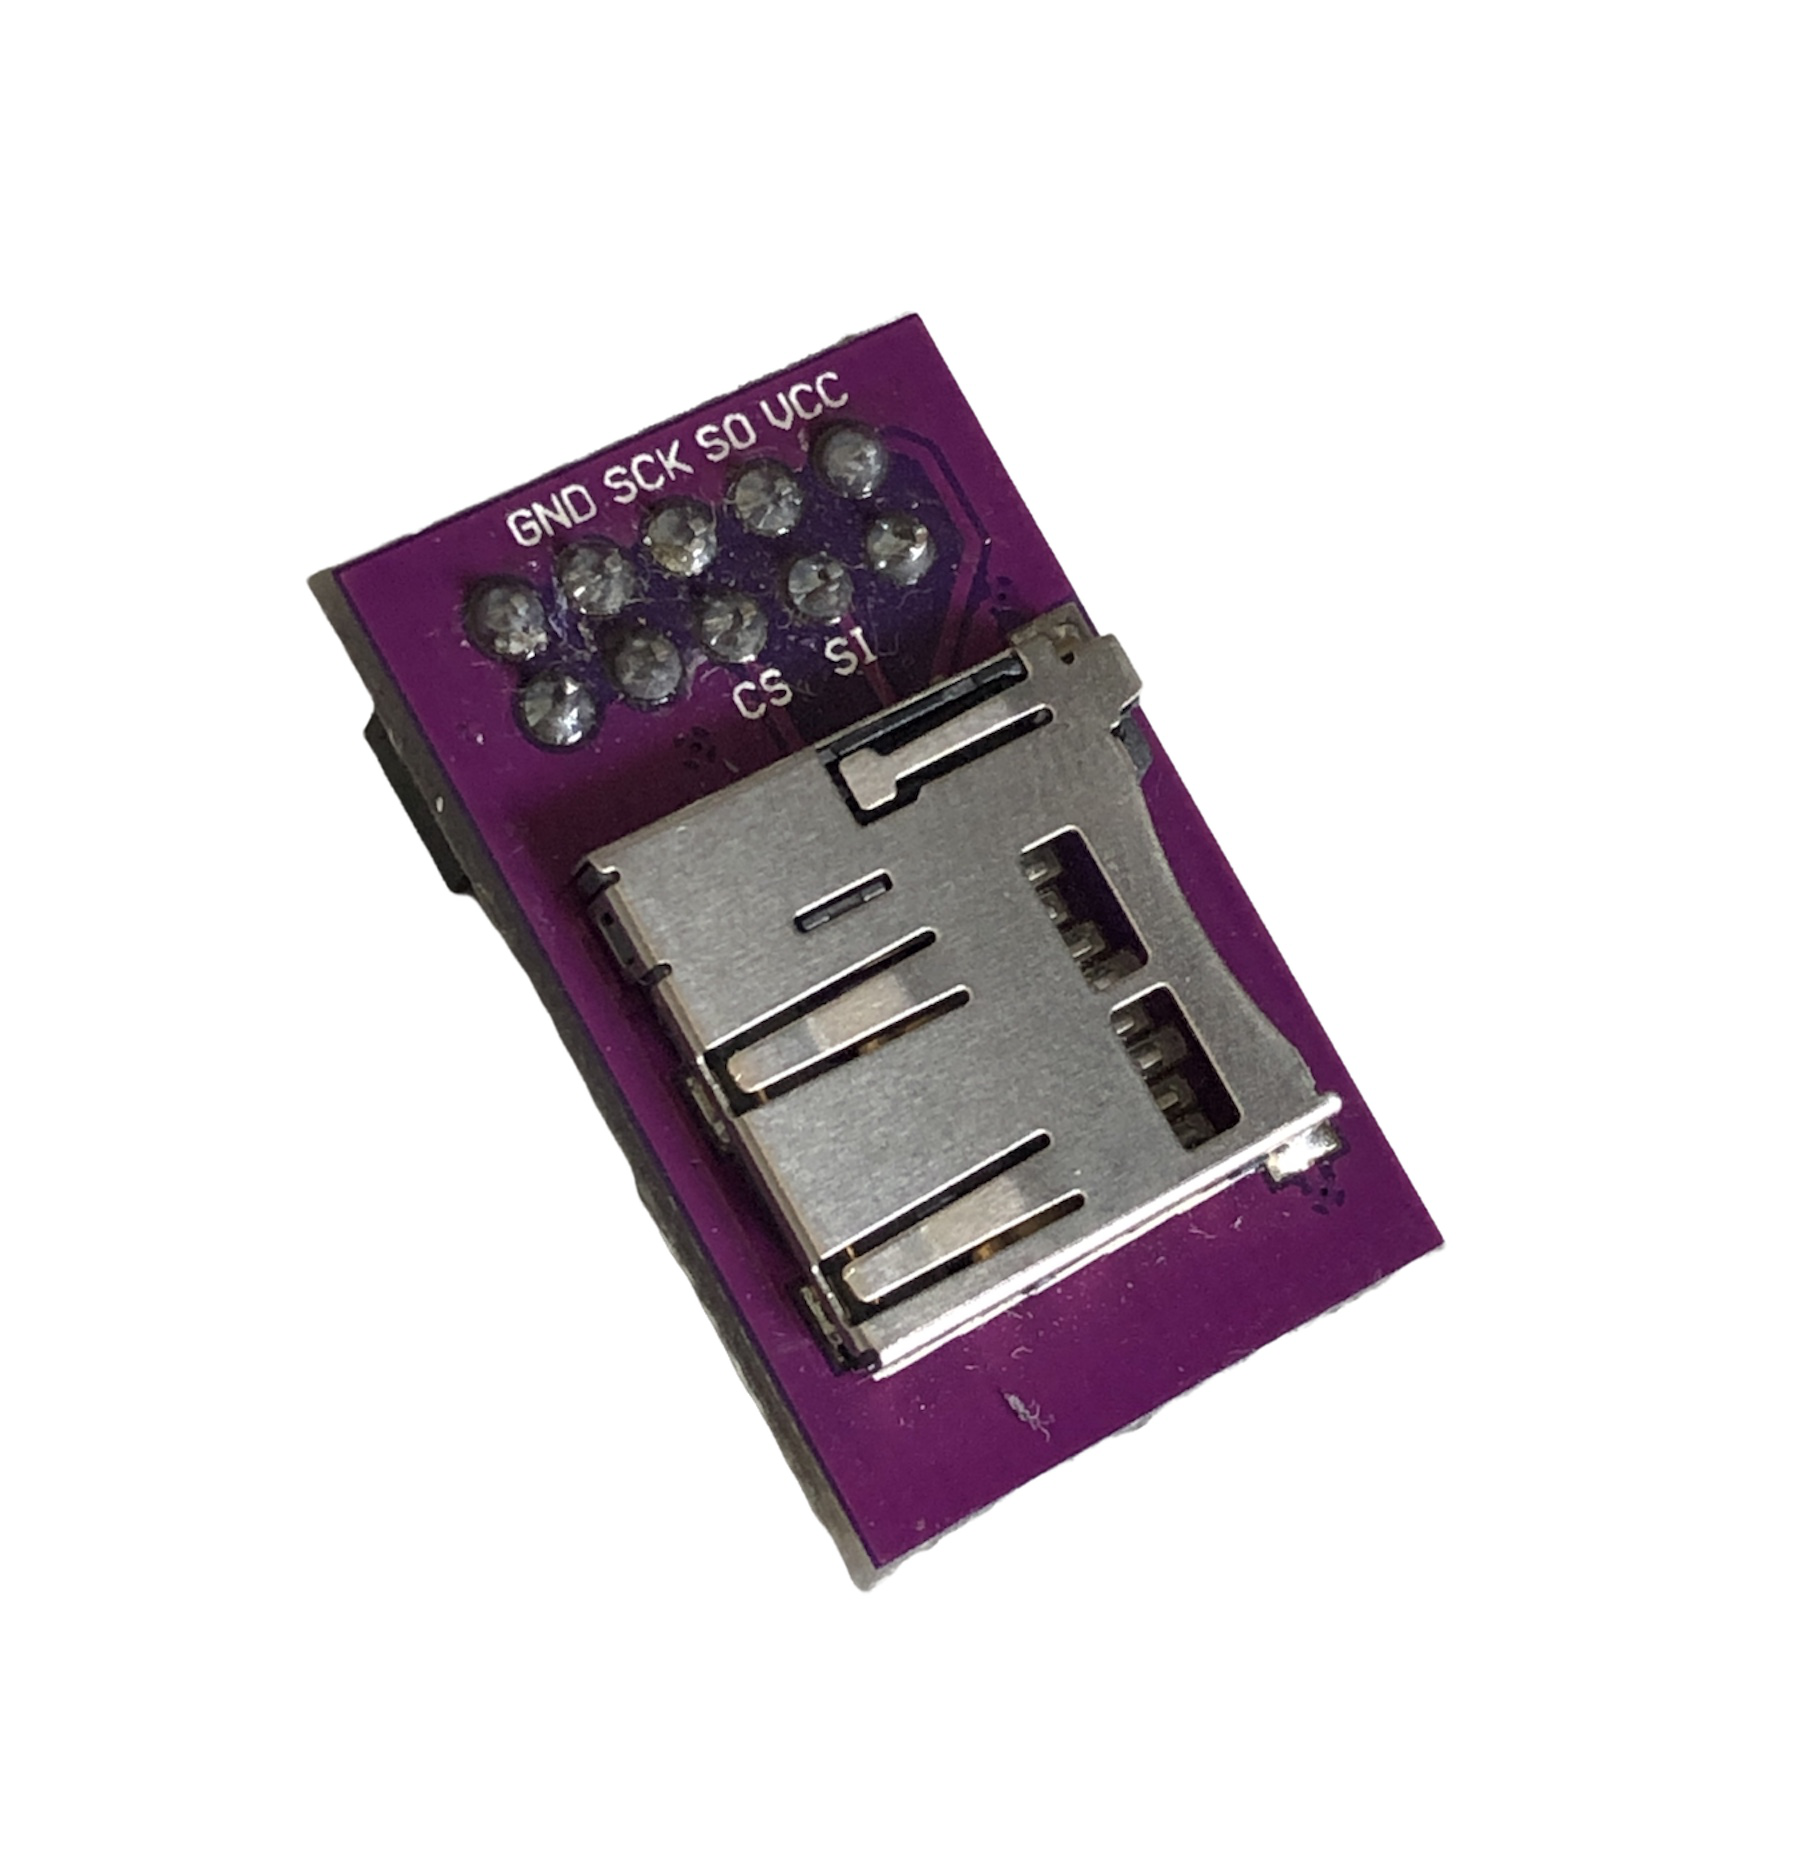
\includegraphics[width=0.6\linewidth]{fig/KY-018/zdj_modułu/front.png}
  \caption{Tył modułu}
  \label{fig:sub2}
\end{subfigure}
\caption{Poglądowe zdjęcia modułu}
\label{fig:test}
\end{figure}

Moduł działa dla napięcia z zakresu 2-5.5V, czas reakcji to około 60ms. Posiada wbudowaną diodę LED, sygnalizującą dotyk. Pojemność kondensatora C1 definiuje czułość.
\begin{figure}[h!]
  \centering
  \includegraphics[width=0.8\linewidth]{fig/KY-018/zasada_dzialania/dotyk.png}
  \caption{Schemat elektryczny TTP223}
  \label{fig:sub1}
\end{figure}
% Please add the following required packages to your document preamble:
% \usepackage{graphicx}
\vspace{0.5cm}

\newpage
\section*{Użycie czujnika}
Ważnym elementem czujnika są dwie zworki, oznaczone na module jako A oraz B. Zwarcie ich ze sobą w róznych kombinacjach pozwala na uzyskanie czterech różnych trybów pracy, co zwiększa uniwersalność i użyteczność samego podzespołu.

\begin{figure}[h!]
  \centering
  \includegraphics[width=0.25\linewidth]{fig/KY-018/zdj_modułu/zworki.png}
  \caption{Lokalizacja zworek}
  \label{fig:sub1}
\end{figure}
% Please add the following required packages to your document preamble:
% \usepackage{graphicx}
\vspace{0.5cm}
\begin{table}[h!]
\centering
\resizebox{\textwidth}{!}{%
\begin{tabular}{|c|c|c|}
\hline
\textbf{A} & \textbf{B} & \textbf{Funkcja}                               \\ \hline
0          & 0          & Wyjście wysokiego poziomu TTL bez blokady      \\ \hline
0          & 1          & Samoblokujący wysoki poziom TTL (pamięć stanu) \\ \hline
1          & 0          & Wyjście niskiego poziomu TTL bez blokady       \\ \hline
1          & 1          & Samoblokujący niski poziom TTL (pamięć stanu)  \\ \hline
\end{tabular}%
}
\caption{\label{tab:table-name}Opis trybów pracy modułu}
\end{table}
Po wyboru jednego z trybów pracy, wystarczy podłączyć moduł do mikroprocesora przez pin cyfrowy. Należy pamiętać, że czułość modułu można dowolnie dostosowywać za pomocą pojemności kondensatora w zakresie 0-50 pf, gdzie 0 pf to maksymalna czułość, a 50 pf to najniższa. Ma to swoje zastosowanie w przypadku, gdy czujnik znajduje się za jakąś osłoną, przykładowo ze szkła lub akrylu; dostosowując czułość czujnika do grubości materiału zapewniamy jego prawidłowe funkcjonowanie (czujnik nie musi być bezpośrednio dotknięty, by wysłał sygnał, działa on na zbliżenie palca do oznaczonej powierzchni). 


\begin{figure}[h!]
\centering
\begin{subfigure}{.5\textwidth}
  \centering
  \includegraphics[width=0.74\linewidth]{fig/KY-018/działanie_ukladu/nie dziala.jpg}
  \caption{Brak interakcji z przyciskiem}
  \label{fig:sub1}
\end{subfigure}%
\begin{subfigure}{.5\textwidth}
  \centering
  \includegraphics[width=0.74\linewidth]{fig/KY-018/działanie_ukladu/dziala.jpg}
  \caption{Dotknięcie przycisku - zapalone diody}
  \label{fig:sub2}
\end{subfigure}
\caption{Poglądowe działanie modułu}
\label{fig:test}
\end{figure}



\newpage

Kod programujący czujnik, wykorzystany do opracowania instrukcji, znajduje się w materiałach dodatkowych zawartych pod koniec rozdziału.
\newline

Film prezentujący działanie układu znajduje się w suplemencie wideo.

\printbibliography[heading=bibintoc]

\end{document}